\documentclass[1p]{elsarticle_modified}
%\bibliographystyle{elsarticle-num}

%\usepackage[colorlinks]{hyperref}
%\usepackage{abbrmath_seonhwa} %\Abb, \Ascr, \Acal ,\Abf, \Afrak
\usepackage{amsfonts}
\usepackage{amssymb}
\usepackage{amsmath}
\usepackage{amsthm}
\usepackage{scalefnt}
\usepackage{amsbsy}
\usepackage{kotex}
\usepackage{caption}
\usepackage{subfig}
\usepackage{color}
\usepackage{graphicx}
\usepackage{xcolor} %% white, black, red, green, blue, cyan, magenta, yellow
\usepackage{float}
\usepackage{setspace}
\usepackage{hyperref}

\usepackage{tikz}
\usetikzlibrary{arrows}

\usepackage{multirow}
\usepackage{array} % fixed length table
\usepackage{hhline}

%%%%%%%%%%%%%%%%%%%%%
\makeatletter
\renewcommand*\env@matrix[1][\arraystretch]{%
	\edef\arraystretch{#1}%
	\hskip -\arraycolsep
	\let\@ifnextchar\new@ifnextchar
	\array{*\c@MaxMatrixCols c}}
\makeatother %https://tex.stackexchange.com/questions/14071/how-can-i-increase-the-line-spacing-in-a-matrix
%%%%%%%%%%%%%%%

\usepackage[normalem]{ulem}

\newcommand{\msout}[1]{\ifmmode\text{\sout{\ensuremath{#1}}}\else\sout{#1}\fi}
%SOURCE: \msout is \stkout macro in https://tex.stackexchange.com/questions/20609/strikeout-in-math-mode

\newcommand{\cancel}[1]{
	\ifmmode
	{\color{red}\msout{#1}}
	\else
	{\color{red}\sout{#1}}
	\fi
}

\newcommand{\add}[1]{
	{\color{blue}\uwave{#1}}
}

\newcommand{\replace}[2]{
	\ifmmode
	{\color{red}\msout{#1}}{\color{blue}\uwave{#2}}
	\else
	{\color{red}\sout{#1}}{\color{blue}\uwave{#2}}
	\fi
}

\newcommand{\Sol}{\mathcal{S}} %segment
\newcommand{\D}{D} %diagram
\newcommand{\A}{\mathcal{A}} %arc


%%%%%%%%%%%%%%%%%%%%%%%%%%%%%5 test

\def\sl{\operatorname{\textup{SL}}(2,\Cbb)}
\def\psl{\operatorname{\textup{PSL}}(2,\Cbb)}
\def\quan{\mkern 1mu \triangleright \mkern 1mu}

\theoremstyle{definition}
\newtheorem{thm}{Theorem}[section]
\newtheorem{prop}[thm]{Proposition}
\newtheorem{lem}[thm]{Lemma}
\newtheorem{ques}[thm]{Question}
\newtheorem{cor}[thm]{Corollary}
\newtheorem{defn}[thm]{Definition}
\newtheorem{exam}[thm]{Example}
\newtheorem{rmk}[thm]{Remark}
\newtheorem{alg}[thm]{Algorithm}

\newcommand{\I}{\sqrt{-1}}
\begin{document}

%\begin{frontmatter}
%
%\title{Boundary parabolic representations of knots up to 8 crossings}
%
%%% Group authors per affiliation:
%\author{Yunhi Cho} 
%\address{Department of Mathematics, University of Seoul, Seoul, Korea}
%\ead{yhcho@uos.ac.kr}
%
%
%\author{Seonhwa Kim} %\fnref{s_kim}}
%\address{Center for Geometry and Physics, Institute for Basic Science, Pohang, 37673, Korea}
%\ead{ryeona17@ibs.re.kr}
%
%\author{Hyuk Kim}
%\address{Department of Mathematical Sciences, Seoul National University, Seoul 08826, Korea}
%\ead{hyukkim@snu.ac.kr}
%
%\author{Seokbeom Yoon}
%\address{Department of Mathematical Sciences, Seoul National University, Seoul, 08826,  Korea}
%\ead{sbyoon15@snu.ac.kr}
%
%\begin{abstract}
%We find all boundary parabolic representation of knots up to 8 crossings.
%
%\end{abstract}
%\begin{keyword}
%    \MSC[2010] 57M25 
%\end{keyword}
%
%\end{frontmatter}

%\linenumbers
%\tableofcontents
%
\newcommand\colored[1]{\textcolor{white}{\rule[-0.35ex]{0.8em}{1.4ex}}\kern-0.8em\color{red} #1}%
%\newcommand\colored[1]{\textcolor{white}{ #1}\kern-2.17ex	\textcolor{white}{ #1}\kern-1.81ex	\textcolor{white}{ #1}\kern-2.15ex\color{red}#1	}

{\Large $\underline{12n_{0834}~(K12n_{0834})}$}

\setlength{\tabcolsep}{10pt}
\renewcommand{\arraystretch}{1.6}
\vspace{1cm}\begin{tabular}{m{100pt}>{\centering\arraybackslash}m{274pt}}
\multirow{5}{120pt}{
	\centering
	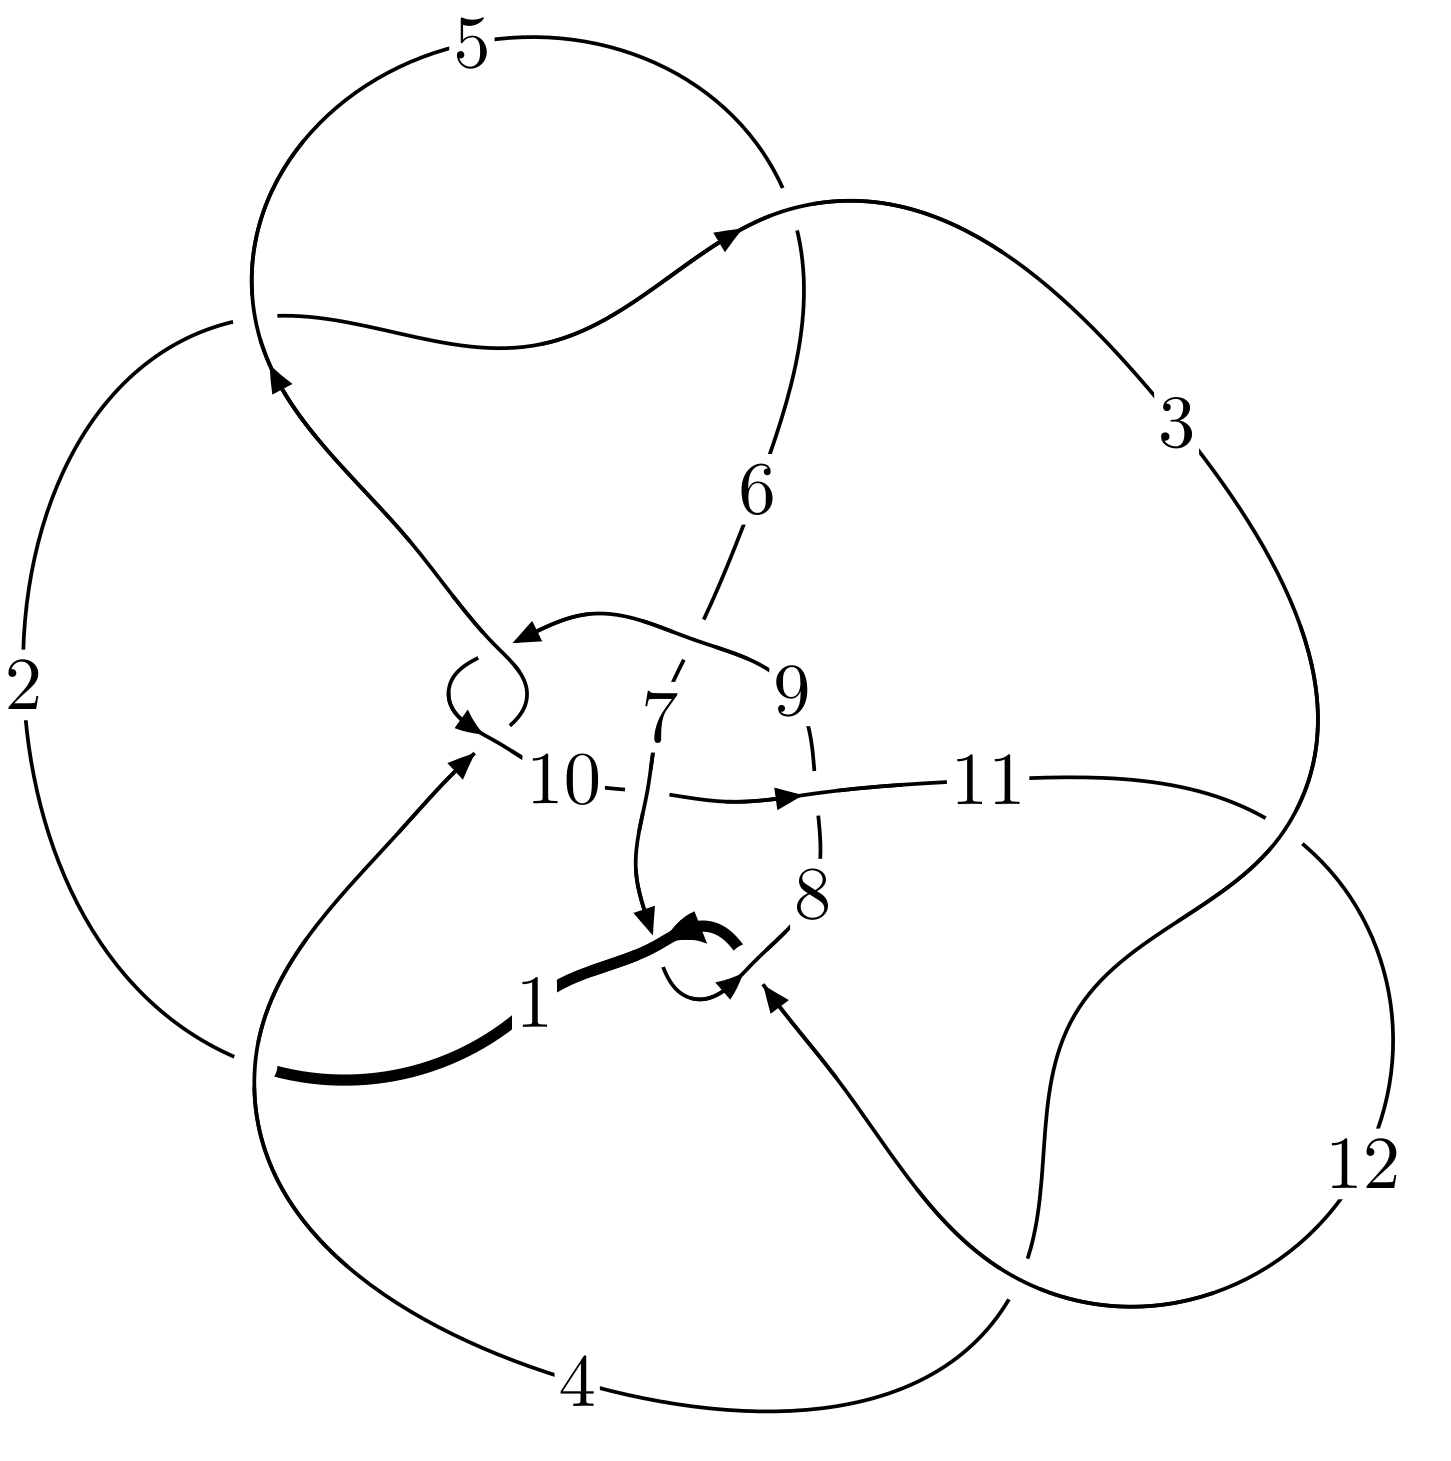
\includegraphics[width=112pt]{../../../GIT/diagram.site/Diagrams/png/2923_12n_0834.png}\\
\ \ \ A knot diagram\footnotemark}&
\allowdisplaybreaks
\textbf{Linearized knot diagam} \\
\cline{2-2}
 &
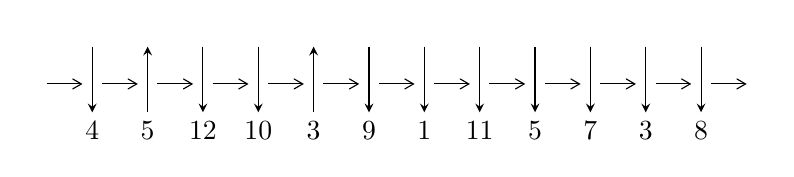
\begin{tikzpicture}[x=20pt, y=17pt]
	% nodes
	\node (C0) at (0, 0) {};
	\node (C1) at (1, 0) {};
	\node (C1U) at (1, +1) {};
	\node (C1D) at (1, -1) {4};

	\node (C2) at (2, 0) {};
	\node (C2U) at (2, +1) {};
	\node (C2D) at (2, -1) {5};

	\node (C3) at (3, 0) {};
	\node (C3U) at (3, +1) {};
	\node (C3D) at (3, -1) {12};

	\node (C4) at (4, 0) {};
	\node (C4U) at (4, +1) {};
	\node (C4D) at (4, -1) {10};

	\node (C5) at (5, 0) {};
	\node (C5U) at (5, +1) {};
	\node (C5D) at (5, -1) {3};

	\node (C6) at (6, 0) {};
	\node (C6U) at (6, +1) {};
	\node (C6D) at (6, -1) {9};

	\node (C7) at (7, 0) {};
	\node (C7U) at (7, +1) {};
	\node (C7D) at (7, -1) {1};

	\node (C8) at (8, 0) {};
	\node (C8U) at (8, +1) {};
	\node (C8D) at (8, -1) {11};

	\node (C9) at (9, 0) {};
	\node (C9U) at (9, +1) {};
	\node (C9D) at (9, -1) {5};

	\node (C10) at (10, 0) {};
	\node (C10U) at (10, +1) {};
	\node (C10D) at (10, -1) {7};

	\node (C11) at (11, 0) {};
	\node (C11U) at (11, +1) {};
	\node (C11D) at (11, -1) {3};

	\node (C12) at (12, 0) {};
	\node (C12U) at (12, +1) {};
	\node (C12D) at (12, -1) {8};
	\node (C13) at (13, 0) {};

	% arrows
	\draw[->,>={angle 60}]
	(C0) edge (C1) (C1) edge (C2) (C2) edge (C3) (C3) edge (C4) (C4) edge (C5) (C5) edge (C6) (C6) edge (C7) (C7) edge (C8) (C8) edge (C9) (C9) edge (C10) (C10) edge (C11) (C11) edge (C12) (C12) edge (C13) ;	\draw[->,>=stealth]
	(C1U) edge (C1D) (C2D) edge (C2U) (C3U) edge (C3D) (C4U) edge (C4D) (C5D) edge (C5U) (C6U) edge (C6D) (C7U) edge (C7D) (C8U) edge (C8D) (C9U) edge (C9D) (C10U) edge (C10D) (C11U) edge (C11D) (C12U) edge (C12D) ;
	\end{tikzpicture} \\
\hhline{~~} \\& 
\textbf{Solving Sequence} \\ \cline{2-2} 
 &
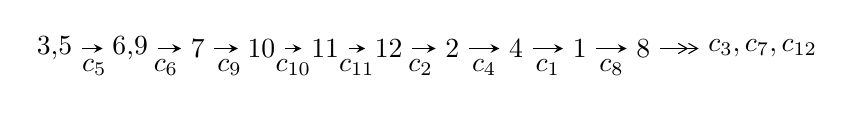
\begin{tikzpicture}[x=23pt, y=7pt]
	% node
	\node (A0) at (-1/8, 0) {3,5};
	\node (A1) at (17/16, 0) {6,9};
	\node (A2) at (17/8, 0) {7};
	\node (A3) at (25/8, 0) {10};
	\node (A4) at (33/8, 0) {11};
	\node (A5) at (41/8, 0) {12};
	\node (A6) at (49/8, 0) {2};
	\node (A7) at (57/8, 0) {4};
	\node (A8) at (65/8, 0) {1};
	\node (A9) at (73/8, 0) {8};
	\node (C1) at (1/2, -1) {$c_{5}$};
	\node (C2) at (13/8, -1) {$c_{6}$};
	\node (C3) at (21/8, -1) {$c_{9}$};
	\node (C4) at (29/8, -1) {$c_{10}$};
	\node (C5) at (37/8, -1) {$c_{11}$};
	\node (C6) at (45/8, -1) {$c_{2}$};
	\node (C7) at (53/8, -1) {$c_{4}$};
	\node (C8) at (61/8, -1) {$c_{1}$};
	\node (C9) at (69/8, -1) {$c_{8}$};
	\node (A10) at (11, 0) {$c_{3},c_{7},c_{12}$};

	% edge
	\draw[->,>=stealth]	
	(A0) edge (A1) (A1) edge (A2) (A2) edge (A3) (A3) edge (A4) (A4) edge (A5) (A5) edge (A6) (A6) edge (A7) (A7) edge (A8) (A8) edge (A9) ;
	\draw[->>,>={angle 60}]	
	(A9) edge (A10);
\end{tikzpicture} \\ 

\end{tabular} \\

\footnotetext{
The image of knot diagram is generated by the software ``\textbf{Draw programme}" developed by Andrew Bartholomew(\url{http://www.layer8.co.uk/maths/draw/index.htm\#Running-draw}), where we modified some parts for our purpose(\url{https://github.com/CATsTAILs/LinksPainter}).
}\phantom \\ \newline 
\centering \textbf{Ideals for irreducible components\footnotemark of $X_{\text{par}}$} 
 
\begin{align*}
I^u_{1}&=\langle 
-1.08966\times10^{500} u^{82}-2.94352\times10^{500} u^{81}+\cdots+5.30022\times10^{505} b-6.35080\times10^{505},\\
\phantom{I^u_{1}}&\phantom{= \langle  }-3.64438\times10^{506} u^{82}-1.00895\times10^{507} u^{81}+\cdots+9.03577\times10^{510} a-1.96606\times10^{512},\\
\phantom{I^u_{1}}&\phantom{= \langle  }u^{83}+3 u^{82}+\cdots+2662084 u+170479\rangle \\
I^u_{2}&=\langle 
-4.04393\times10^{21} u^{26}+1.97112\times10^{22} u^{25}+\cdots+1.93265\times10^{20} b-3.76256\times10^{21},\\
\phantom{I^u_{2}}&\phantom{= \langle  }1.42730\times10^{21} u^{26}-6.73395\times10^{21} u^{25}+\cdots+1.93265\times10^{20} a+2.32727\times10^{20},\;u^{27}-4 u^{26}+\cdots-6 u+1\rangle \\
\\
\end{align*}
\raggedright * 2 irreducible components of $\dim_{\mathbb{C}}=0$, with total 110 representations.\\
\footnotetext{All coefficients of polynomials are rational numbers. But the coefficients are sometimes approximated in decimal forms when there is not enough margin.}
\newpage
\renewcommand{\arraystretch}{1}
\centering \section*{I. $I^u_{1}= \langle -1.09\times10^{500} u^{82}-2.94\times10^{500} u^{81}+\cdots+5.30\times10^{505} b-6.35\times10^{505},\;-3.64\times10^{506} u^{82}-1.01\times10^{507} u^{81}+\cdots+9.04\times10^{510} a-1.97\times10^{512},\;u^{83}+3 u^{82}+\cdots+2662084 u+170479 \rangle$}
\flushleft \textbf{(i) Arc colorings}\\
\begin{tabular}{m{7pt} m{180pt} m{7pt} m{180pt} }
\flushright $a_{3}=$&$\begin{pmatrix}0\\u\end{pmatrix}$ \\
\flushright $a_{5}=$&$\begin{pmatrix}1\\0\end{pmatrix}$ \\
\flushright $a_{6}=$&$\begin{pmatrix}1\\- u^2\end{pmatrix}$ \\
\flushright $a_{9}=$&$\begin{pmatrix}0.0000403328 u^{82}+0.000111662 u^{81}+\cdots+301.582 u+21.7586\\2.05587\times10^{-6} u^{82}+5.55358\times10^{-6} u^{81}+\cdots+16.7884 u+1.19821\end{pmatrix}$ \\
\flushright $a_{7}=$&$\begin{pmatrix}7.99165\times10^{-6} u^{82}+0.0000218152 u^{81}+\cdots+83.4879 u+11.2783\\3.56446\times10^{-6} u^{82}+8.91911\times10^{-6} u^{81}+\cdots+12.5852 u+1.13575\end{pmatrix}$ \\
\flushright $a_{10}=$&$\begin{pmatrix}0.0000382770 u^{82}+0.000106108 u^{81}+\cdots+284.794 u+20.5604\\2.05587\times10^{-6} u^{82}+5.55358\times10^{-6} u^{81}+\cdots+16.7884 u+1.19821\end{pmatrix}$ \\
\flushright $a_{11}=$&$\begin{pmatrix}0.0000270188 u^{82}+0.0000765238 u^{81}+\cdots+263.798 u+21.3036\\3.76716\times10^{-6} u^{82}+9.89186\times10^{-6} u^{81}+\cdots+26.9027 u+2.10980\end{pmatrix}$ \\
\flushright $a_{12}=$&$\begin{pmatrix}0.0000270188 u^{82}+0.0000765238 u^{81}+\cdots+263.798 u+21.3036\\4.37821\times10^{-6} u^{82}+0.0000117106 u^{81}+\cdots+34.3627 u+2.88251\end{pmatrix}$ \\
\flushright $a_{2}=$&$\begin{pmatrix}- u\\u\end{pmatrix}$ \\
\flushright $a_{4}=$&$\begin{pmatrix}-8.47736\times10^{-6} u^{82}-0.0000243217 u^{81}+\cdots-110.183 u-10.6747\\-2.67993\times10^{-6} u^{82}-6.44923\times10^{-6} u^{81}+\cdots-7.29709 u-0.675289\end{pmatrix}$ \\
\flushright $a_{1}=$&$\begin{pmatrix}9.13713\times10^{-6} u^{82}+0.0000248460 u^{81}+\cdots+28.5787 u+2.02038\\8.20590\times10^{-6} u^{82}+0.0000216780 u^{81}+\cdots+38.0155 u+2.21423\end{pmatrix}$ \\
\flushright $a_{8}=$&$\begin{pmatrix}0.0000343092 u^{82}+0.0000920768 u^{81}+\cdots+221.021 u+17.7205\\-1.53610\times10^{-6} u^{82}-5.91305\times10^{-6} u^{81}+\cdots-34.4259 u-2.76913\end{pmatrix}$\\&\end{tabular}
\flushleft \textbf{(ii) Obstruction class $= -1$}\\~\\
\flushleft \textbf{(iii) Cusp Shapes $= -0.0000735631 u^{82}-0.000207254 u^{81}+\cdots-607.762 u-56.2513$}\\~\\
\newpage\renewcommand{\arraystretch}{1}
\flushleft \textbf{(iv) u-Polynomials at the component}\newline \\
\begin{tabular}{m{50pt}|m{274pt}}
Crossings & \hspace{64pt}u-Polynomials at each crossing \\
\hline $$\begin{aligned}c_{1}\end{aligned}$$&$\begin{aligned}
&u^{83}-3 u^{82}+\cdots+348287054 u+1799981
\end{aligned}$\\
\hline $$\begin{aligned}c_{2},c_{5}\end{aligned}$$&$\begin{aligned}
&u^{83}+3 u^{82}+\cdots+2662084 u+170479
\end{aligned}$\\
\hline $$\begin{aligned}c_{3},c_{11}\end{aligned}$$&$\begin{aligned}
&u^{83}+2 u^{82}+\cdots+6280 u+317
\end{aligned}$\\
\hline $$\begin{aligned}c_{4},c_{9}\end{aligned}$$&$\begin{aligned}
&u^{83}+u^{82}+\cdots+355 u^2+19
\end{aligned}$\\
\hline $$\begin{aligned}c_{6}\end{aligned}$$&$\begin{aligned}
&u^{83}-10 u^{82}+\cdots-5710543466 u+554133157
\end{aligned}$\\
\hline $$\begin{aligned}c_{7},c_{12}\end{aligned}$$&$\begin{aligned}
&u^{83}- u^{82}+\cdots-94 u+421
\end{aligned}$\\
\hline $$\begin{aligned}c_{8}\end{aligned}$$&$\begin{aligned}
&u^{83}-2 u^{82}+\cdots+2794 u+4489
\end{aligned}$\\
\hline $$\begin{aligned}c_{10}\end{aligned}$$&$\begin{aligned}
&u^{83}+u^{82}+\cdots-9 u+1
\end{aligned}$\\
\hline
\end{tabular}\\~\\
\newpage\renewcommand{\arraystretch}{1}
\flushleft \textbf{(v) Riley Polynomials at the component}\newline \\
\begin{tabular}{m{50pt}|m{274pt}}
Crossings & \hspace{64pt}Riley Polynomials at each crossing \\
\hline $$\begin{aligned}c_{1}\end{aligned}$$&$\begin{aligned}
&y^{83}-67 y^{82}+\cdots+126569059795229812 y-3239931600361
\end{aligned}$\\
\hline $$\begin{aligned}c_{2},c_{5}\end{aligned}$$&$\begin{aligned}
&y^{83}+73 y^{82}+\cdots+763249377340 y-29063089441
\end{aligned}$\\
\hline $$\begin{aligned}c_{3},c_{11}\end{aligned}$$&$\begin{aligned}
&y^{83}-52 y^{82}+\cdots+9384264 y-100489
\end{aligned}$\\
\hline $$\begin{aligned}c_{4},c_{9}\end{aligned}$$&$\begin{aligned}
&y^{83}+25 y^{82}+\cdots-13490 y-361
\end{aligned}$\\
\hline $$\begin{aligned}c_{6}\end{aligned}$$&$\begin{aligned}
&y^{83}-104 y^{82}+\cdots+9.99\times10^{18} y-3.07\times10^{17}
\end{aligned}$\\
\hline $$\begin{aligned}c_{7},c_{12}\end{aligned}$$&$\begin{aligned}
&y^{83}+51 y^{82}+\cdots-4179272 y-177241
\end{aligned}$\\
\hline $$\begin{aligned}c_{8}\end{aligned}$$&$\begin{aligned}
&y^{83}-14 y^{82}+\cdots+313731786 y-20151121
\end{aligned}$\\
\hline $$\begin{aligned}c_{10}\end{aligned}$$&$\begin{aligned}
&y^{83}+7 y^{82}+\cdots+19 y-1
\end{aligned}$\\
\hline
\end{tabular}\\~\\
\newpage\flushleft \textbf{(vi) Complex Volumes and Cusp Shapes}
$$\begin{array}{c|c|c}  
\text{Solutions to }I^u_{1}& \I (\text{vol} + \sqrt{-1}CS) & \text{Cusp shape}\\
 \hline 
\begin{aligned}
u &= \phantom{-}0.460170 + 0.898995 I \\
a &= -0.168620 + 0.726275 I \\
b &= -0.221048 + 0.705863 I\end{aligned}
 & \phantom{-}4.26133 - 0.63411 I & \phantom{-0.000000 } 0 \\ \hline\begin{aligned}
u &= \phantom{-}0.460170 - 0.898995 I \\
a &= -0.168620 - 0.726275 I \\
b &= -0.221048 - 0.705863 I\end{aligned}
 & \phantom{-}4.26133 + 0.63411 I & \phantom{-0.000000 } 0 \\ \hline\begin{aligned}
u &= -0.941883 + 0.232685 I \\
a &= \phantom{-}0.197853 - 0.761878 I \\
b &= -0.06542 + 1.55250 I\end{aligned}
 & \phantom{-}9.22626 - 0.03282 I & \phantom{-0.000000 } 0 \\ \hline\begin{aligned}
u &= -0.941883 - 0.232685 I \\
a &= \phantom{-}0.197853 + 0.761878 I \\
b &= -0.06542 - 1.55250 I\end{aligned}
 & \phantom{-}9.22626 + 0.03282 I & \phantom{-0.000000 } 0 \\ \hline\begin{aligned}
u &= \phantom{-}0.151233 + 1.055790 I \\
a &= -1.63266 - 0.24668 I \\
b &= -0.669200 + 0.693855 I\end{aligned}
 & -3.59693 - 0.25964 I & \phantom{-0.000000 } 0 \\ \hline\begin{aligned}
u &= \phantom{-}0.151233 - 1.055790 I \\
a &= -1.63266 + 0.24668 I \\
b &= -0.669200 - 0.693855 I\end{aligned}
 & -3.59693 + 0.25964 I & \phantom{-0.000000 } 0 \\ \hline\begin{aligned}
u &= \phantom{-}0.104503 + 0.894745 I \\
a &= -1.48586 + 0.41944 I \\
b &= \phantom{-}0.130955 + 0.330576 I\end{aligned}
 & -1.93363 + 2.55099 I & -6.08801 - 4.34231 I \\ \hline\begin{aligned}
u &= \phantom{-}0.104503 - 0.894745 I \\
a &= -1.48586 - 0.41944 I \\
b &= \phantom{-}0.130955 - 0.330576 I\end{aligned}
 & -1.93363 - 2.55099 I & -6.08801 + 4.34231 I \\ \hline\begin{aligned}
u &= -0.320146 + 0.834261 I \\
a &= \phantom{-}0.32192 - 1.66448 I \\
b &= -0.061384 - 0.907535 I\end{aligned}
 & \phantom{-}2.46760 + 6.12253 I & -5.10820 - 3.57469 I \\ \hline\begin{aligned}
u &= -0.320146 - 0.834261 I \\
a &= \phantom{-}0.32192 + 1.66448 I \\
b &= -0.061384 + 0.907535 I\end{aligned}
 & \phantom{-}2.46760 - 6.12253 I & -5.10820 + 3.57469 I\\
 \hline 
 \end{array}$$\newpage$$\begin{array}{c|c|c}  
\text{Solutions to }I^u_{1}& \I (\text{vol} + \sqrt{-1}CS) & \text{Cusp shape}\\
 \hline 
\begin{aligned}
u &= -1.079120 + 0.323083 I \\
a &= -0.102641 - 1.048010 I \\
b &= -0.002580 + 0.402975 I\end{aligned}
 & \phantom{-}4.68534 - 3.54286 I & \phantom{-0.000000 } 0 \\ \hline\begin{aligned}
u &= -1.079120 - 0.323083 I \\
a &= -0.102641 + 1.048010 I \\
b &= -0.002580 - 0.402975 I\end{aligned}
 & \phantom{-}4.68534 + 3.54286 I & \phantom{-0.000000 } 0 \\ \hline\begin{aligned}
u &= \phantom{-}0.766720 + 0.305993 I \\
a &= -0.152016 + 0.363218 I \\
b &= -0.072957 + 1.226830 I\end{aligned}
 & \phantom{-}7.80934 + 4.18853 I & \phantom{-}5.53622 - 8.64057 I \\ \hline\begin{aligned}
u &= \phantom{-}0.766720 - 0.305993 I \\
a &= -0.152016 - 0.363218 I \\
b &= -0.072957 - 1.226830 I\end{aligned}
 & \phantom{-}7.80934 - 4.18853 I & \phantom{-}5.53622 + 8.64057 I \\ \hline\begin{aligned}
u &= \phantom{-}0.361275 + 0.737742 I \\
a &= \phantom{-}0.647299 + 0.280234 I \\
b &= -0.15977 - 1.58744 I\end{aligned}
 & \phantom{-}2.95977 - 5.59698 I & -7.31611 + 4.13920 I \\ \hline\begin{aligned}
u &= \phantom{-}0.361275 - 0.737742 I \\
a &= \phantom{-}0.647299 - 0.280234 I \\
b &= -0.15977 + 1.58744 I\end{aligned}
 & \phantom{-}2.95977 + 5.59698 I & -7.31611 - 4.13920 I \\ \hline\begin{aligned}
u &= \phantom{-}0.800505 + 0.047194 I \\
a &= \phantom{-}0.0794772 - 0.0099353 I \\
b &= \phantom{-}0.191222 - 0.999614 I\end{aligned}
 & \phantom{-}2.00895 + 1.88550 I & -2.97510 - 3.95787 I \\ \hline\begin{aligned}
u &= \phantom{-}0.800505 - 0.047194 I \\
a &= \phantom{-}0.0794772 + 0.0099353 I \\
b &= \phantom{-}0.191222 + 0.999614 I\end{aligned}
 & \phantom{-}2.00895 - 1.88550 I & -2.97510 + 3.95787 I \\ \hline\begin{aligned}
u &= \phantom{-}0.153357 + 1.222420 I \\
a &= \phantom{-}1.209470 - 0.126486 I \\
b &= \phantom{-}0.692358 - 0.502979 I\end{aligned}
 & -1.37477 + 2.01127 I & \phantom{-0.000000 } 0 \\ \hline\begin{aligned}
u &= \phantom{-}0.153357 - 1.222420 I \\
a &= \phantom{-}1.209470 + 0.126486 I \\
b &= \phantom{-}0.692358 + 0.502979 I\end{aligned}
 & -1.37477 - 2.01127 I & \phantom{-0.000000 } 0\\
 \hline 
 \end{array}$$\newpage$$\begin{array}{c|c|c}  
\text{Solutions to }I^u_{1}& \I (\text{vol} + \sqrt{-1}CS) & \text{Cusp shape}\\
 \hline 
\begin{aligned}
u &= -0.767881 + 0.006018 I \\
a &= \phantom{-}0.684140 - 0.442889 I \\
b &= -0.932129 - 0.022458 I\end{aligned}
 & -3.25081 - 0.95000 I & -7.88321 + 7.61599 I \\ \hline\begin{aligned}
u &= -0.767881 - 0.006018 I \\
a &= \phantom{-}0.684140 + 0.442889 I \\
b &= -0.932129 + 0.022458 I\end{aligned}
 & -3.25081 + 0.95000 I & -7.88321 - 7.61599 I \\ \hline\begin{aligned}
u &= \phantom{-}0.549190 + 1.115550 I \\
a &= \phantom{-}1.300670 - 0.214187 I \\
b &= \phantom{-}0.588894 - 0.776860 I\end{aligned}
 & -0.96511 + 2.32927 I & \phantom{-0.000000 } 0 \\ \hline\begin{aligned}
u &= \phantom{-}0.549190 - 1.115550 I \\
a &= \phantom{-}1.300670 + 0.214187 I \\
b &= \phantom{-}0.588894 + 0.776860 I\end{aligned}
 & -0.96511 - 2.32927 I & \phantom{-0.000000 } 0 \\ \hline\begin{aligned}
u &= -0.685812 + 0.256869 I \\
a &= -0.389456 + 0.622000 I \\
b &= \phantom{-}0.786038 - 0.201636 I\end{aligned}
 & -2.43520 + 2.07800 I & -9.07465 - 2.81903 I \\ \hline\begin{aligned}
u &= -0.685812 - 0.256869 I \\
a &= -0.389456 - 0.622000 I \\
b &= \phantom{-}0.786038 + 0.201636 I\end{aligned}
 & -2.43520 - 2.07800 I & -9.07465 + 2.81903 I \\ \hline\begin{aligned}
u &= \phantom{-}0.240184 + 1.253840 I \\
a &= -1.32154 + 0.54080 I \\
b &= -0.669629 + 1.120710 I\end{aligned}
 & -2.11921 + 5.33902 I & \phantom{-0.000000 } 0 \\ \hline\begin{aligned}
u &= \phantom{-}0.240184 - 1.253840 I \\
a &= -1.32154 - 0.54080 I \\
b &= -0.669629 - 1.120710 I\end{aligned}
 & -2.11921 - 5.33902 I & \phantom{-0.000000 } 0 \\ \hline\begin{aligned}
u &= -0.452391 + 1.200180 I \\
a &= -1.327090 + 0.475985 I \\
b &= -1.124410 - 0.597252 I\end{aligned}
 & -6.01531 - 1.51859 I & \phantom{-0.000000 } 0 \\ \hline\begin{aligned}
u &= -0.452391 - 1.200180 I \\
a &= -1.327090 - 0.475985 I \\
b &= -1.124410 + 0.597252 I\end{aligned}
 & -6.01531 + 1.51859 I & \phantom{-0.000000 } 0\\
 \hline 
 \end{array}$$\newpage$$\begin{array}{c|c|c}  
\text{Solutions to }I^u_{1}& \I (\text{vol} + \sqrt{-1}CS) & \text{Cusp shape}\\
 \hline 
\begin{aligned}
u &= \phantom{-}0.559073 + 0.326140 I \\
a &= -0.091237 - 0.446252 I \\
b &= \phantom{-}0.338905 + 1.330250 I\end{aligned}
 & \phantom{-}1.39029 - 2.51273 I & -5.26385 - 4.80671 I \\ \hline\begin{aligned}
u &= \phantom{-}0.559073 - 0.326140 I \\
a &= -0.091237 + 0.446252 I \\
b &= \phantom{-}0.338905 - 1.330250 I\end{aligned}
 & \phantom{-}1.39029 + 2.51273 I & -5.26385 + 4.80671 I \\ \hline\begin{aligned}
u &= \phantom{-}1.262080 + 0.619347 I \\
a &= -0.080706 + 0.577363 I \\
b &= -0.267607 - 1.101350 I\end{aligned}
 & \phantom{-}2.47880 + 4.31907 I & \phantom{-0.000000 } 0 \\ \hline\begin{aligned}
u &= \phantom{-}1.262080 - 0.619347 I \\
a &= -0.080706 - 0.577363 I \\
b &= -0.267607 + 1.101350 I\end{aligned}
 & \phantom{-}2.47880 - 4.31907 I & \phantom{-0.000000 } 0 \\ \hline\begin{aligned}
u &= -0.303827 + 1.372880 I \\
a &= \phantom{-}1.302350 - 0.009523 I \\
b &= \phantom{-}1.34178 + 1.06457 I\end{aligned}
 & -7.37820 - 4.65827 I & \phantom{-0.000000 } 0 \\ \hline\begin{aligned}
u &= -0.303827 - 1.372880 I \\
a &= \phantom{-}1.302350 + 0.009523 I \\
b &= \phantom{-}1.34178 - 1.06457 I\end{aligned}
 & -7.37820 + 4.65827 I & \phantom{-0.000000 } 0 \\ \hline\begin{aligned}
u &= \phantom{-}0.50902 + 1.34890 I \\
a &= -0.938167 - 0.437644 I \\
b &= -0.744424 + 1.131700 I\end{aligned}
 & -3.23576 + 0.65655 I & \phantom{-0.000000 } 0 \\ \hline\begin{aligned}
u &= \phantom{-}0.50902 - 1.34890 I \\
a &= -0.938167 + 0.437644 I \\
b &= -0.744424 - 1.131700 I\end{aligned}
 & -3.23576 - 0.65655 I & \phantom{-0.000000 } 0 \\ \hline\begin{aligned}
u &= \phantom{-}0.316164 + 0.450393 I \\
a &= -2.61551 + 2.38499 I \\
b &= -0.515805 + 0.697975 I\end{aligned}
 & \phantom{-}1.42765 + 8.76014 I & -8.9252 - 11.6486 I \\ \hline\begin{aligned}
u &= \phantom{-}0.316164 - 0.450393 I \\
a &= -2.61551 - 2.38499 I \\
b &= -0.515805 - 0.697975 I\end{aligned}
 & \phantom{-}1.42765 - 8.76014 I & -8.9252 + 11.6486 I\\
 \hline 
 \end{array}$$\newpage$$\begin{array}{c|c|c}  
\text{Solutions to }I^u_{1}& \I (\text{vol} + \sqrt{-1}CS) & \text{Cusp shape}\\
 \hline 
\begin{aligned}
u &= -0.526776 + 0.130625 I \\
a &= \phantom{-}1.64907 + 1.42838 I \\
b &= -0.063525 + 0.410583 I\end{aligned}
 & -1.212250 + 0.458419 I & -8.45009 + 2.61399 I \\ \hline\begin{aligned}
u &= -0.526776 - 0.130625 I \\
a &= \phantom{-}1.64907 - 1.42838 I \\
b &= -0.063525 - 0.410583 I\end{aligned}
 & -1.212250 - 0.458419 I & -8.45009 - 2.61399 I \\ \hline\begin{aligned}
u &= -0.04934 + 1.49667 I \\
a &= -0.934626 - 0.361125 I \\
b &= -0.95732 - 1.26988 I\end{aligned}
 & -4.02002 - 6.07736 I & \phantom{-0.000000 } 0 \\ \hline\begin{aligned}
u &= -0.04934 - 1.49667 I \\
a &= -0.934626 + 0.361125 I \\
b &= -0.95732 + 1.26988 I\end{aligned}
 & -4.02002 + 6.07736 I & \phantom{-0.000000 } 0 \\ \hline\begin{aligned}
u &= \phantom{-}1.42390 + 0.51355 I \\
a &= \phantom{-}1.40096 + 0.28358 I \\
b &= \phantom{-}0.410299 - 0.847136 I\end{aligned}
 & -1.12191 + 2.28952 I & \phantom{-0.000000 } 0 \\ \hline\begin{aligned}
u &= \phantom{-}1.42390 - 0.51355 I \\
a &= \phantom{-}1.40096 - 0.28358 I \\
b &= \phantom{-}0.410299 + 0.847136 I\end{aligned}
 & -1.12191 - 2.28952 I & \phantom{-0.000000 } 0 \\ \hline\begin{aligned}
u &= \phantom{-}0.23379 + 1.55264 I \\
a &= \phantom{-}0.938585 + 0.174861 I \\
b &= \phantom{-}1.11049 - 0.94048 I\end{aligned}
 & -2.12242 - 2.67601 I & \phantom{-0.000000 } 0 \\ \hline\begin{aligned}
u &= \phantom{-}0.23379 - 1.55264 I \\
a &= \phantom{-}0.938585 - 0.174861 I \\
b &= \phantom{-}1.11049 + 0.94048 I\end{aligned}
 & -2.12242 + 2.67601 I & \phantom{-0.000000 } 0 \\ \hline\begin{aligned}
u &= \phantom{-}0.24509 + 1.55456 I \\
a &= \phantom{-}1.245430 - 0.100646 I \\
b &= \phantom{-}0.481804 - 0.886418 I\end{aligned}
 & -0.87721 + 2.01433 I & \phantom{-0.000000 } 0 \\ \hline\begin{aligned}
u &= \phantom{-}0.24509 - 1.55456 I \\
a &= \phantom{-}1.245430 + 0.100646 I \\
b &= \phantom{-}0.481804 + 0.886418 I\end{aligned}
 & -0.87721 - 2.01433 I & \phantom{-0.000000 } 0\\
 \hline 
 \end{array}$$\newpage$$\begin{array}{c|c|c}  
\text{Solutions to }I^u_{1}& \I (\text{vol} + \sqrt{-1}CS) & \text{Cusp shape}\\
 \hline 
\begin{aligned}
u &= -0.51376 + 1.57596 I \\
a &= \phantom{-}0.945701 - 0.164051 I \\
b &= \phantom{-}1.09511 + 1.11076 I\end{aligned}
 & -8.17262 - 4.55804 I & \phantom{-0.000000 } 0 \\ \hline\begin{aligned}
u &= -0.51376 - 1.57596 I \\
a &= \phantom{-}0.945701 + 0.164051 I \\
b &= \phantom{-}1.09511 - 1.11076 I\end{aligned}
 & -8.17262 + 4.55804 I & \phantom{-0.000000 } 0 \\ \hline\begin{aligned}
u &= -0.279421 + 0.154723 I \\
a &= -1.57511 - 2.32845 I \\
b &= \phantom{-}0.391533 - 1.077430 I\end{aligned}
 & \phantom{-}0.89383 + 5.51966 I & -4.81577 - 6.93480 I \\ \hline\begin{aligned}
u &= -0.279421 - 0.154723 I \\
a &= -1.57511 + 2.32845 I \\
b &= \phantom{-}0.391533 + 1.077430 I\end{aligned}
 & \phantom{-}0.89383 - 5.51966 I & -4.81577 + 6.93480 I \\ \hline\begin{aligned}
u &= -0.77897 + 1.52417 I \\
a &= -0.834559 + 0.320224 I \\
b &= -0.83894 - 1.21576 I\end{aligned}
 & -5.57447 - 8.53577 I & \phantom{-0.000000 } 0 \\ \hline\begin{aligned}
u &= -0.77897 - 1.52417 I \\
a &= -0.834559 - 0.320224 I \\
b &= -0.83894 + 1.21576 I\end{aligned}
 & -5.57447 + 8.53577 I & \phantom{-0.000000 } 0 \\ \hline\begin{aligned}
u &= \phantom{-}1.71458 + 0.23735 I \\
a &= \phantom{-}0.024016 + 0.194910 I \\
b &= -0.322108 - 0.323947 I\end{aligned}
 & \phantom{-}4.44720 - 1.98419 I & \phantom{-0.000000 } 0 \\ \hline\begin{aligned}
u &= \phantom{-}1.71458 - 0.23735 I \\
a &= \phantom{-}0.024016 - 0.194910 I \\
b &= -0.322108 + 0.323947 I\end{aligned}
 & \phantom{-}4.44720 + 1.98419 I & \phantom{-0.000000 } 0 \\ \hline\begin{aligned}
u &= \phantom{-}0.29319 + 1.73778 I \\
a &= -0.832574 + 0.208844 I \\
b &= -0.842256 + 0.841665 I\end{aligned}
 & -4.08145 + 5.34949 I & \phantom{-0.000000 } 0 \\ \hline\begin{aligned}
u &= \phantom{-}0.29319 - 1.73778 I \\
a &= -0.832574 - 0.208844 I \\
b &= -0.842256 - 0.841665 I\end{aligned}
 & -4.08145 - 5.34949 I & \phantom{-0.000000 } 0\\
 \hline 
 \end{array}$$\newpage$$\begin{array}{c|c|c}  
\text{Solutions to }I^u_{1}& \I (\text{vol} + \sqrt{-1}CS) & \text{Cusp shape}\\
 \hline 
\begin{aligned}
u &= \phantom{-}0.13010 + 1.76314 I \\
a &= \phantom{-}0.915724 + 0.008694 I \\
b &= \phantom{-}1.25100 + 0.73854 I\end{aligned}
 & -7.22965 + 9.66297 I & \phantom{-0.000000 } 0 \\ \hline\begin{aligned}
u &= \phantom{-}0.13010 - 1.76314 I \\
a &= \phantom{-}0.915724 - 0.008694 I \\
b &= \phantom{-}1.25100 - 0.73854 I\end{aligned}
 & -7.22965 - 9.66297 I & \phantom{-0.000000 } 0 \\ \hline\begin{aligned}
u &= -0.142785 + 0.170899 I \\
a &= -3.16147 - 4.45029 I \\
b &= -0.578288 - 0.452235 I\end{aligned}
 & \phantom{-}3.08537 - 3.61369 I & -6.55201 + 5.17838 I \\ \hline\begin{aligned}
u &= -0.142785 - 0.170899 I \\
a &= -3.16147 + 4.45029 I \\
b &= -0.578288 + 0.452235 I\end{aligned}
 & \phantom{-}3.08537 + 3.61369 I & -6.55201 - 5.17838 I \\ \hline\begin{aligned}
u &= -0.213112\phantom{ +0.000000I} \\
a &= \phantom{-}2.54188\phantom{ +0.000000I} \\
b &= \phantom{-}0.384068\phantom{ +0.000000I}\end{aligned}
 & -0.791810\phantom{ +0.000000I} & -12.6720\phantom{ +0.000000I} \\ \hline\begin{aligned}
u &= \phantom{-}0.08659 + 1.81227 I \\
a &= -0.887978 + 0.026815 I \\
b &= -1.057560 - 0.878142 I\end{aligned}
 & -10.06270 + 3.27636 I & \phantom{-0.000000 } 0 \\ \hline\begin{aligned}
u &= \phantom{-}0.08659 - 1.81227 I \\
a &= -0.887978 - 0.026815 I \\
b &= -1.057560 + 0.878142 I\end{aligned}
 & -10.06270 - 3.27636 I & \phantom{-0.000000 } 0 \\ \hline\begin{aligned}
u &= -0.19032 + 1.80895 I \\
a &= \phantom{-}0.786350 + 0.062928 I \\
b &= \phantom{-}1.16484 + 0.96951 I\end{aligned}
 & -8.59582 - 3.52880 I & \phantom{-0.000000 } 0 \\ \hline\begin{aligned}
u &= -0.19032 - 1.80895 I \\
a &= \phantom{-}0.786350 - 0.062928 I \\
b &= \phantom{-}1.16484 - 0.96951 I\end{aligned}
 & -8.59582 + 3.52880 I & \phantom{-0.000000 } 0 \\ \hline\begin{aligned}
u &= -1.83255 + 0.07076 I \\
a &= -0.200666 + 0.252048 I \\
b &= -0.658066 - 0.537500 I\end{aligned}
 & \phantom{-}0.28249 - 8.18613 I & \phantom{-0.000000 } 0\\
 \hline 
 \end{array}$$\newpage$$\begin{array}{c|c|c}  
\text{Solutions to }I^u_{1}& \I (\text{vol} + \sqrt{-1}CS) & \text{Cusp shape}\\
 \hline 
\begin{aligned}
u &= -1.83255 - 0.07076 I \\
a &= -0.200666 - 0.252048 I \\
b &= -0.658066 + 0.537500 I\end{aligned}
 & \phantom{-}0.28249 + 8.18613 I & \phantom{-0.000000 } 0 \\ \hline\begin{aligned}
u &= \phantom{-}0.51163 + 1.76987 I \\
a &= \phantom{-}0.879156 - 0.064606 I \\
b &= \phantom{-}0.97483 - 1.06910 I\end{aligned}
 & -1.63743 + 10.21140 I & \phantom{-0.000000 } 0 \\ \hline\begin{aligned}
u &= \phantom{-}0.51163 - 1.76987 I \\
a &= \phantom{-}0.879156 + 0.064606 I \\
b &= \phantom{-}0.97483 + 1.06910 I\end{aligned}
 & -1.63743 - 10.21140 I & \phantom{-0.000000 } 0 \\ \hline\begin{aligned}
u &= -1.77339 + 0.64608 I \\
a &= \phantom{-}0.517134 - 0.144678 I \\
b &= \phantom{-}0.519924 + 0.414154 I\end{aligned}
 & -2.58248 - 0.86247 I & \phantom{-0.000000 } 0 \\ \hline\begin{aligned}
u &= -1.77339 - 0.64608 I \\
a &= \phantom{-}0.517134 + 0.144678 I \\
b &= \phantom{-}0.519924 - 0.414154 I\end{aligned}
 & -2.58248 + 0.86247 I & \phantom{-0.000000 } 0 \\ \hline\begin{aligned}
u &= \phantom{-}0.03322 + 1.92914 I \\
a &= -0.648747 - 0.094426 I \\
b &= -1.046470 - 0.645501 I\end{aligned}
 & -7.35769 + 1.59908 I & \phantom{-0.000000 } 0 \\ \hline\begin{aligned}
u &= \phantom{-}0.03322 - 1.92914 I \\
a &= -0.648747 + 0.094426 I \\
b &= -1.046470 + 0.645501 I\end{aligned}
 & -7.35769 - 1.59908 I & \phantom{-0.000000 } 0 \\ \hline\begin{aligned}
u &= -0.73084 + 1.79088 I \\
a &= \phantom{-}0.969017 - 0.067168 I \\
b &= \phantom{-}0.91767 + 1.21902 I\end{aligned}
 & -5.6307 - 17.3815 I & \phantom{-0.000000 } 0 \\ \hline\begin{aligned}
u &= -0.73084 - 1.79088 I \\
a &= \phantom{-}0.969017 + 0.067168 I \\
b &= \phantom{-}0.91767 - 1.21902 I\end{aligned}
 & -5.6307 + 17.3815 I & \phantom{-0.000000 } 0 \\ \hline\begin{aligned}
u &= -0.75604 + 1.88383 I \\
a &= -0.930165 + 0.071600 I \\
b &= -0.922238 - 1.068110 I\end{aligned}
 & -9.40953 - 10.47900 I & \phantom{-0.000000 } 0\\
 \hline 
 \end{array}$$\newpage$$\begin{array}{c|c|c}  
\text{Solutions to }I^u_{1}& \I (\text{vol} + \sqrt{-1}CS) & \text{Cusp shape}\\
 \hline 
\begin{aligned}
u &= -0.75604 - 1.88383 I \\
a &= -0.930165 - 0.071600 I \\
b &= -0.922238 + 1.068110 I\end{aligned}
 & -9.40953 + 10.47900 I & \phantom{-0.000000 } 0 \\ \hline\begin{aligned}
u &= -0.17374 + 2.29146 I \\
a &= \phantom{-}0.880997 - 0.058898 I \\
b &= \phantom{-}0.713431 + 0.936889 I\end{aligned}
 & -2.47728 - 2.75627 I & \phantom{-0.000000 } 0 \\ \hline\begin{aligned}
u &= -0.17374 - 2.29146 I \\
a &= \phantom{-}0.880997 + 0.058898 I \\
b &= \phantom{-}0.713431 - 0.936889 I\end{aligned}
 & -2.47728 + 2.75627 I & \phantom{-0.000000 } 0\\
 \hline 
 \end{array}$$\newpage\newpage\renewcommand{\arraystretch}{1}
\centering \section*{II. $I^u_{2}= \langle -4.04\times10^{21} u^{26}+1.97\times10^{22} u^{25}+\cdots+1.93\times10^{20} b-3.76\times10^{21},\;1.43\times10^{21} u^{26}-6.73\times10^{21} u^{25}+\cdots+1.93\times10^{20} a+2.33\times10^{20},\;u^{27}-4 u^{26}+\cdots-6 u+1 \rangle$}
\flushleft \textbf{(i) Arc colorings}\\
\begin{tabular}{m{7pt} m{180pt} m{7pt} m{180pt} }
\flushright $a_{3}=$&$\begin{pmatrix}0\\u\end{pmatrix}$ \\
\flushright $a_{5}=$&$\begin{pmatrix}1\\0\end{pmatrix}$ \\
\flushright $a_{6}=$&$\begin{pmatrix}1\\- u^2\end{pmatrix}$ \\
\flushright $a_{9}=$&$\begin{pmatrix}-7.38521 u^{26}+34.8432 u^{25}+\cdots+30.8641 u-1.20419\\20.9243 u^{26}-101.991 u^{25}+\cdots-147.137 u+19.4685\end{pmatrix}$ \\
\flushright $a_{7}=$&$\begin{pmatrix}-10.6002 u^{26}+51.6860 u^{25}+\cdots+80.1888 u-6.20606\\20.9788 u^{26}-102.527 u^{25}+\cdots-159.836 u+20.2238\end{pmatrix}$ \\
\flushright $a_{10}=$&$\begin{pmatrix}-28.3095 u^{26}+136.834 u^{25}+\cdots+178.001 u-20.6726\\20.9243 u^{26}-101.991 u^{25}+\cdots-147.137 u+19.4685\end{pmatrix}$ \\
\flushright $a_{11}=$&$\begin{pmatrix}-5.40776 u^{26}+26.0671 u^{25}+\cdots+41.8757 u-0.657312\\-15.4098 u^{26}+76.2735 u^{25}+\cdots+115.483 u-18.5009\end{pmatrix}$ \\
\flushright $a_{12}=$&$\begin{pmatrix}-5.40776 u^{26}+26.0671 u^{25}+\cdots+41.8757 u-0.657312\\-18.7489 u^{26}+92.5673 u^{25}+\cdots+147.508 u-22.9370\end{pmatrix}$ \\
\flushright $a_{2}=$&$\begin{pmatrix}- u\\u\end{pmatrix}$ \\
\flushright $a_{4}=$&$\begin{pmatrix}58.0982 u^{26}-284.534 u^{25}+\cdots-452.283 u+58.5015\\-37.6519 u^{26}+184.309 u^{25}+\cdots+290.925 u-38.6642\end{pmatrix}$ \\
\flushright $a_{1}=$&$\begin{pmatrix}-0.594465 u^{26}+3.26250 u^{25}+\cdots+17.0575 u-0.276555\\-9.02856 u^{26}+44.5812 u^{25}+\cdots+69.3910 u-10.7702\end{pmatrix}$ \\
\flushright $a_{8}=$&$\begin{pmatrix}8.01099 u^{26}-39.0436 u^{25}+\cdots-63.6642 u+15.2616\\11.1766 u^{26}-54.5617 u^{25}+\cdots-86.0744 u+9.40541\end{pmatrix}$\\&\end{tabular}
\flushleft \textbf{(ii) Obstruction class $= 1$}\\~\\
\flushleft \textbf{(iii) Cusp Shapes $= -\frac{33323838254448526961075}{193264588372002970811} u^{26}+\frac{164472182050612511766757}{193264588372002970811} u^{25}+\cdots+\frac{270764044802687883745440}{193264588372002970811} u-\frac{41347340969186927752163}{193264588372002970811}$}\\~\\
\newpage\renewcommand{\arraystretch}{1}
\flushleft \textbf{(iv) u-Polynomials at the component}\newline \\
\begin{tabular}{m{50pt}|m{274pt}}
Crossings & \hspace{64pt}u-Polynomials at each crossing \\
\hline $$\begin{aligned}c_{1}\end{aligned}$$&$\begin{aligned}
&u^{27}-12 u^{26}+\cdots-8 u-229
\end{aligned}$\\
\hline $$\begin{aligned}c_{2}\end{aligned}$$&$\begin{aligned}
&u^{27}+4 u^{26}+\cdots-6 u-1
\end{aligned}$\\
\hline $$\begin{aligned}c_{3}\end{aligned}$$&$\begin{aligned}
&u^{27}-5 u^{26}+\cdots-6 u+1
\end{aligned}$\\
\hline $$\begin{aligned}c_{4}\end{aligned}$$&$\begin{aligned}
&u^{27}+2 u^{26}+\cdots-13 u^2-1
\end{aligned}$\\
\hline $$\begin{aligned}c_{5}\end{aligned}$$&$\begin{aligned}
&u^{27}-4 u^{26}+\cdots-6 u+1
\end{aligned}$\\
\hline $$\begin{aligned}c_{6}\end{aligned}$$&$\begin{aligned}
&u^{27}- u^{26}+\cdots+336 u-173
\end{aligned}$\\
\hline $$\begin{aligned}c_{7}\end{aligned}$$&$\begin{aligned}
&u^{27}-2 u^{26}+\cdots+2 u+1
\end{aligned}$\\
\hline $$\begin{aligned}c_{8}\end{aligned}$$&$\begin{aligned}
&u^{27}- u^{26}+\cdots-2 u-1
\end{aligned}$\\
\hline $$\begin{aligned}c_{9}\end{aligned}$$&$\begin{aligned}
&u^{27}-2 u^{26}+\cdots+13 u^2+1
\end{aligned}$\\
\hline $$\begin{aligned}c_{10}\end{aligned}$$&$\begin{aligned}
&u^{27}+5 u^{25}+\cdots+7 u+1
\end{aligned}$\\
\hline $$\begin{aligned}c_{11}\end{aligned}$$&$\begin{aligned}
&u^{27}+5 u^{26}+\cdots-6 u-1
\end{aligned}$\\
\hline $$\begin{aligned}c_{12}\end{aligned}$$&$\begin{aligned}
&u^{27}+2 u^{26}+\cdots+2 u-1
\end{aligned}$\\
\hline
\end{tabular}\\~\\
\newpage\renewcommand{\arraystretch}{1}
\flushleft \textbf{(v) Riley Polynomials at the component}\newline \\
\begin{tabular}{m{50pt}|m{274pt}}
Crossings & \hspace{64pt}Riley Polynomials at each crossing \\
\hline $$\begin{aligned}c_{1}\end{aligned}$$&$\begin{aligned}
&y^{27}-20 y^{26}+\cdots+1415284 y-52441
\end{aligned}$\\
\hline $$\begin{aligned}c_{2},c_{5}\end{aligned}$$&$\begin{aligned}
&y^{27}+16 y^{24}+\cdots+28 y-1
\end{aligned}$\\
\hline $$\begin{aligned}c_{3},c_{11}\end{aligned}$$&$\begin{aligned}
&y^{27}-9 y^{26}+\cdots+20 y-1
\end{aligned}$\\
\hline $$\begin{aligned}c_{4},c_{9}\end{aligned}$$&$\begin{aligned}
&y^{27}+20 y^{26}+\cdots-26 y-1
\end{aligned}$\\
\hline $$\begin{aligned}c_{6}\end{aligned}$$&$\begin{aligned}
&y^{27}+31 y^{26}+\cdots+67570 y-29929
\end{aligned}$\\
\hline $$\begin{aligned}c_{7},c_{12}\end{aligned}$$&$\begin{aligned}
&y^{27}+22 y^{26}+\cdots-40 y^2-1
\end{aligned}$\\
\hline $$\begin{aligned}c_{8}\end{aligned}$$&$\begin{aligned}
&y^{27}+9 y^{26}+\cdots+6 y-1
\end{aligned}$\\
\hline $$\begin{aligned}c_{10}\end{aligned}$$&$\begin{aligned}
&y^{27}+10 y^{26}+\cdots+39 y-1
\end{aligned}$\\
\hline
\end{tabular}\\~\\
\newpage\flushleft \textbf{(vi) Complex Volumes and Cusp Shapes}
$$\begin{array}{c|c|c}  
\text{Solutions to }I^u_{2}& \I (\text{vol} + \sqrt{-1}CS) & \text{Cusp shape}\\
 \hline 
\begin{aligned}
u &= \phantom{-}0.011508 + 0.960762 I \\
a &= -1.59813 + 0.58298 I \\
b &= -0.158063 + 0.354673 I\end{aligned}
 & -3.28117 + 2.00579 I & -13.62403 - 3.47473 I \\ \hline\begin{aligned}
u &= \phantom{-}0.011508 - 0.960762 I \\
a &= -1.59813 - 0.58298 I \\
b &= -0.158063 - 0.354673 I\end{aligned}
 & -3.28117 - 2.00579 I & -13.62403 + 3.47473 I \\ \hline\begin{aligned}
u &= -1.026840 + 0.248737 I \\
a &= -1.107710 - 0.660114 I \\
b &= \phantom{-}0.170360 - 0.749462 I\end{aligned}
 & \phantom{-}2.07996 + 7.57439 I & -4.21001 - 7.63313 I \\ \hline\begin{aligned}
u &= -1.026840 - 0.248737 I \\
a &= -1.107710 + 0.660114 I \\
b &= \phantom{-}0.170360 + 0.749462 I\end{aligned}
 & \phantom{-}2.07996 - 7.57439 I & -4.21001 + 7.63313 I \\ \hline\begin{aligned}
u &= -0.910768 + 0.010715 I \\
a &= -0.212195 + 0.911198 I \\
b &= \phantom{-}0.08610 - 1.55715 I\end{aligned}
 & \phantom{-}9.18890 - 0.57633 I & -5.5467 + 13.1274 I \\ \hline\begin{aligned}
u &= -0.910768 - 0.010715 I \\
a &= -0.212195 - 0.911198 I \\
b &= \phantom{-}0.08610 + 1.55715 I\end{aligned}
 & \phantom{-}9.18890 + 0.57633 I & -5.5467 - 13.1274 I \\ \hline\begin{aligned}
u &= -0.901824\phantom{ +0.000000I} \\
a &= -0.122321\phantom{ +0.000000I} \\
b &= \phantom{-}0.805064\phantom{ +0.000000I}\end{aligned}
 & -3.43153\phantom{ +0.000000I} & -12.0740\phantom{ +0.000000I} \\ \hline\begin{aligned}
u &= \phantom{-}1.097310 + 0.319632 I \\
a &= -0.165655 + 1.075010 I \\
b &= -0.017250 - 0.689297 I\end{aligned}
 & \phantom{-}5.14703 + 3.51083 I & \phantom{-}3.22862 - 1.62442 I \\ \hline\begin{aligned}
u &= \phantom{-}1.097310 - 0.319632 I \\
a &= -0.165655 - 1.075010 I \\
b &= -0.017250 + 0.689297 I\end{aligned}
 & \phantom{-}5.14703 - 3.51083 I & \phantom{-}3.22862 + 1.62442 I \\ \hline\begin{aligned}
u &= \phantom{-}0.403986 + 1.079340 I \\
a &= -1.27045 - 0.63545 I \\
b &= -0.766066 + 0.866289 I\end{aligned}
 & -2.36848 - 0.53520 I & -6.99550 + 1.26697 I\\
 \hline 
 \end{array}$$\newpage$$\begin{array}{c|c|c}  
\text{Solutions to }I^u_{2}& \I (\text{vol} + \sqrt{-1}CS) & \text{Cusp shape}\\
 \hline 
\begin{aligned}
u &= \phantom{-}0.403986 - 1.079340 I \\
a &= -1.27045 + 0.63545 I \\
b &= -0.766066 - 0.866289 I\end{aligned}
 & -2.36848 + 0.53520 I & -6.99550 - 1.26697 I \\ \hline\begin{aligned}
u &= -0.200525 + 1.237720 I \\
a &= \phantom{-}1.389760 - 0.042816 I \\
b &= \phantom{-}0.471583 - 1.001310 I\end{aligned}
 & -0.73876 + 1.53239 I & -13.14639 + 3.16974 I \\ \hline\begin{aligned}
u &= -0.200525 - 1.237720 I \\
a &= \phantom{-}1.389760 + 0.042816 I \\
b &= \phantom{-}0.471583 + 1.001310 I\end{aligned}
 & -0.73876 - 1.53239 I & -13.14639 - 3.16974 I \\ \hline\begin{aligned}
u &= \phantom{-}0.087914 + 1.261540 I \\
a &= -1.093090 + 0.703743 I \\
b &= -0.713641 + 1.066830 I\end{aligned}
 & -1.56049 + 6.01678 I & -6.76815 - 9.06378 I \\ \hline\begin{aligned}
u &= \phantom{-}0.087914 - 1.261540 I \\
a &= -1.093090 - 0.703743 I \\
b &= -0.713641 - 1.066830 I\end{aligned}
 & -1.56049 - 6.01678 I & -6.76815 + 9.06378 I \\ \hline\begin{aligned}
u &= \phantom{-}0.687795 + 0.149655 I \\
a &= -1.42021 - 0.58787 I \\
b &= \phantom{-}0.046892 + 1.311860 I\end{aligned}
 & \phantom{-}4.43619 + 6.56592 I & -2.27593 - 6.29860 I \\ \hline\begin{aligned}
u &= \phantom{-}0.687795 - 0.149655 I \\
a &= -1.42021 + 0.58787 I \\
b &= \phantom{-}0.046892 - 1.311860 I\end{aligned}
 & \phantom{-}4.43619 - 6.56592 I & -2.27593 + 6.29860 I \\ \hline\begin{aligned}
u &= -0.618893 + 0.275049 I \\
a &= -0.079398 - 0.928011 I \\
b &= -0.080572 - 1.247090 I\end{aligned}
 & \phantom{-}7.44583 - 3.94798 I & -10.42204 - 1.37695 I \\ \hline\begin{aligned}
u &= -0.618893 - 0.275049 I \\
a &= -0.079398 + 0.928011 I \\
b &= -0.080572 + 1.247090 I\end{aligned}
 & \phantom{-}7.44583 + 3.94798 I & -10.42204 + 1.37695 I \\ \hline\begin{aligned}
u &= -0.33613 + 1.40789 I \\
a &= -1.189530 + 0.025816 I \\
b &= -1.31239 - 1.09984 I\end{aligned}
 & -7.06890 - 4.61624 I & \phantom{-}1.56312 + 2.77810 I\\
 \hline 
 \end{array}$$\newpage$$\begin{array}{c|c|c}  
\text{Solutions to }I^u_{2}& \I (\text{vol} + \sqrt{-1}CS) & \text{Cusp shape}\\
 \hline 
\begin{aligned}
u &= -0.33613 - 1.40789 I \\
a &= -1.189530 - 0.025816 I \\
b &= -1.31239 + 1.09984 I\end{aligned}
 & -7.06890 + 4.61624 I & \phantom{-}1.56312 - 2.77810 I \\ \hline\begin{aligned}
u &= \phantom{-}1.55547 + 0.37415 I \\
a &= -0.203973 + 0.071367 I \\
b &= \phantom{-}0.211811 + 0.536233 I\end{aligned}
 & \phantom{-}4.79550 - 2.02115 I & \phantom{-0.000000 } 0 \\ \hline\begin{aligned}
u &= \phantom{-}1.55547 - 0.37415 I \\
a &= -0.203973 - 0.071367 I \\
b &= \phantom{-}0.211811 - 0.536233 I\end{aligned}
 & \phantom{-}4.79550 + 2.02115 I & \phantom{-0.000000 } 0 \\ \hline\begin{aligned}
u &= \phantom{-}0.228176 + 0.104580 I \\
a &= \phantom{-}0.20393 - 2.73007 I \\
b &= \phantom{-}0.192012 + 1.320610 I\end{aligned}
 & \phantom{-}1.24796 - 3.09784 I & -8.17629 + 7.75380 I \\ \hline\begin{aligned}
u &= \phantom{-}0.228176 - 0.104580 I \\
a &= \phantom{-}0.20393 + 2.73007 I \\
b &= \phantom{-}0.192012 - 1.320610 I\end{aligned}
 & \phantom{-}1.24796 + 3.09784 I & -8.17629 - 7.75380 I \\ \hline\begin{aligned}
u &= \phantom{-}1.47191 + 1.30625 I \\
a &= \phantom{-}1.307810 + 0.070078 I \\
b &= \phantom{-}0.466693 - 0.859632 I\end{aligned}
 & -1.15846 + 2.18965 I & \phantom{-0.000000 } 0 \\ \hline\begin{aligned}
u &= \phantom{-}1.47191 - 1.30625 I \\
a &= \phantom{-}1.307810 - 0.070078 I \\
b &= \phantom{-}0.466693 + 0.859632 I\end{aligned}
 & -1.15846 - 2.18965 I & \phantom{-0.000000 } 0\\
 \hline 
 \end{array}$$\newpage
\newpage\renewcommand{\arraystretch}{1}
\centering \section*{ III. u-Polynomials}
\begin{tabular}{m{50pt}|m{274pt}}
Crossings & \hspace{64pt}u-Polynomials at each crossing \\
\hline $$\begin{aligned}c_{1}\end{aligned}$$&$\begin{aligned}
&(u^{27}-12 u^{26}+\cdots-8 u-229)\\
&\cdot(u^{83}-3 u^{82}+\cdots+348287054 u+1799981)
\end{aligned}$\\
\hline $$\begin{aligned}c_{2}\end{aligned}$$&$\begin{aligned}
&(u^{27}+4 u^{26}+\cdots-6 u-1)(u^{83}+3 u^{82}+\cdots+2662084 u+170479)
\end{aligned}$\\
\hline $$\begin{aligned}c_{3}\end{aligned}$$&$\begin{aligned}
&(u^{27}-5 u^{26}+\cdots-6 u+1)(u^{83}+2 u^{82}+\cdots+6280 u+317)
\end{aligned}$\\
\hline $$\begin{aligned}c_{4}\end{aligned}$$&$\begin{aligned}
&(u^{27}+2 u^{26}+\cdots-13 u^2-1)(u^{83}+u^{82}+\cdots+355 u^2+19)
\end{aligned}$\\
\hline $$\begin{aligned}c_{5}\end{aligned}$$&$\begin{aligned}
&(u^{27}-4 u^{26}+\cdots-6 u+1)(u^{83}+3 u^{82}+\cdots+2662084 u+170479)
\end{aligned}$\\
\hline $$\begin{aligned}c_{6}\end{aligned}$$&$\begin{aligned}
&(u^{27}- u^{26}+\cdots+336 u-173)\\
&\cdot(u^{83}-10 u^{82}+\cdots-5710543466 u+554133157)
\end{aligned}$\\
\hline $$\begin{aligned}c_{7}\end{aligned}$$&$\begin{aligned}
&(u^{27}-2 u^{26}+\cdots+2 u+1)(u^{83}- u^{82}+\cdots-94 u+421)
\end{aligned}$\\
\hline $$\begin{aligned}c_{8}\end{aligned}$$&$\begin{aligned}
&(u^{27}- u^{26}+\cdots-2 u-1)(u^{83}-2 u^{82}+\cdots+2794 u+4489)
\end{aligned}$\\
\hline $$\begin{aligned}c_{9}\end{aligned}$$&$\begin{aligned}
&(u^{27}-2 u^{26}+\cdots+13 u^2+1)(u^{83}+u^{82}+\cdots+355 u^2+19)
\end{aligned}$\\
\hline $$\begin{aligned}c_{10}\end{aligned}$$&$\begin{aligned}
&(u^{27}+5 u^{25}+\cdots+7 u+1)(u^{83}+u^{82}+\cdots-9 u+1)
\end{aligned}$\\
\hline $$\begin{aligned}c_{11}\end{aligned}$$&$\begin{aligned}
&(u^{27}+5 u^{26}+\cdots-6 u-1)(u^{83}+2 u^{82}+\cdots+6280 u+317)
\end{aligned}$\\
\hline $$\begin{aligned}c_{12}\end{aligned}$$&$\begin{aligned}
&(u^{27}+2 u^{26}+\cdots+2 u-1)(u^{83}- u^{82}+\cdots-94 u+421)
\end{aligned}$\\
\hline
\end{tabular}\newpage\renewcommand{\arraystretch}{1}
\centering \section*{ IV. Riley Polynomials}
\begin{tabular}{m{50pt}|m{274pt}}
Crossings & \hspace{64pt}Riley Polynomials at each crossing \\
\hline $$\begin{aligned}c_{1}\end{aligned}$$&$\begin{aligned}
&(y^{27}-20 y^{26}+\cdots+1415284 y-52441)\\
&\cdot(y^{83}-67 y^{82}+\cdots+126569059795229812 y-3239931600361)
\end{aligned}$\\
\hline $$\begin{aligned}c_{2},c_{5}\end{aligned}$$&$\begin{aligned}
&(y^{27}+16 y^{24}+\cdots+28 y-1)\\
&\cdot(y^{83}+73 y^{82}+\cdots+763249377340 y-29063089441)
\end{aligned}$\\
\hline $$\begin{aligned}c_{3},c_{11}\end{aligned}$$&$\begin{aligned}
&(y^{27}-9 y^{26}+\cdots+20 y-1)(y^{83}-52 y^{82}+\cdots+9384264 y-100489)
\end{aligned}$\\
\hline $$\begin{aligned}c_{4},c_{9}\end{aligned}$$&$\begin{aligned}
&(y^{27}+20 y^{26}+\cdots-26 y-1)(y^{83}+25 y^{82}+\cdots-13490 y-361)
\end{aligned}$\\
\hline $$\begin{aligned}c_{6}\end{aligned}$$&$\begin{aligned}
&(y^{27}+31 y^{26}+\cdots+67570 y-29929)\\
&\cdot(y^{83}-104 y^{82}+\cdots+9.99\times10^{18} y-3.07\times10^{17})
\end{aligned}$\\
\hline $$\begin{aligned}c_{7},c_{12}\end{aligned}$$&$\begin{aligned}
&(y^{27}+22 y^{26}+\cdots-40 y^2-1)\\
&\cdot(y^{83}+51 y^{82}+\cdots-4179272 y-177241)
\end{aligned}$\\
\hline $$\begin{aligned}c_{8}\end{aligned}$$&$\begin{aligned}
&(y^{27}+9 y^{26}+\cdots+6 y-1)\\
&\cdot(y^{83}-14 y^{82}+\cdots+313731786 y-20151121)
\end{aligned}$\\
\hline $$\begin{aligned}c_{10}\end{aligned}$$&$\begin{aligned}
&(y^{27}+10 y^{26}+\cdots+39 y-1)(y^{83}+7 y^{82}+\cdots+19 y-1)
\end{aligned}$\\
\hline
\end{tabular}
\vskip 2pc
\end{document}